
%%% Local Variables:
%%% mode: latex
%%% TeX-master: t
%%% End:

\chapter{索引结构综述}
\label{cha:related-work}
前文已经提到,近邻查询问题最关键的就是如何选取出一个待选集合$S'$。为了高效地删选出待选集合,我们通常会先把原始的数据索引起来。依据
索引结构的不同,近邻查询的方法可以分为基于树结构的索引和基于哈希的索引。
\section{基于树结构的索引}
\subsection{KD-树}
\subsection{K-Means树}
\section{基于哈希的索引}
基于哈希的索引方法是将高维的数据压缩成二进制编码的形式来进行近似近邻查询,这类方法在图像、文本、视频等多媒体检索上取得不错的效果。
根据哈希函数形式的不同,我们可以简单地将哈希索引分为两类——汉明嵌入和向量量化。
\subsection{汉明嵌入}
汉明嵌入就是要寻找一个映射,对于任意的对象$x \in S$都能映射到二进制串$b(x) \in {0,1}^d$。那么,任意两个对象之间的相似度就可以通过
其对应二进制串之间的汉明距离来近似计算:
\begin{equation}
sim(x, y)\thickapprox 1 - \frac{2\delta_{Ham}(b(x),b(y))}{d}
\end{equation}
\subsection{向量量化}
基于向量量化的哈希索引是对原始向量空间进行量化压缩,原始向量$\mathbf{x} \in \mathbb{R}^D$ 通过量化函数 $q$ 被映射到 $q(\mathbf{x}) \in \mathcal{C} = \{\mathbf{c}_i\}$,其中 $i$ 是下标,$\mathbf{c}_i$ 可以称作为码字,而$\mathcal{C}$则被称为码本。 这种映射可以形式化定义成:$\forall \mathbf{x} \in \mathbb{R}^D$,$\exists \mathbf{c}_i \in \mathcal{C} $,$q(\mathbf{x})=\mathbf{c}_i$。整个量化过程中的量化误差 $E$ 就可以定义为:
\begin{equation}
E = \frac{1}{n}\sum_{\mathbf{x}}\lVert \mathbf{x} - q(\mathbf{x}) \rVert ^2
\end{equation}

其中$\lVert \cdot \rVert$ 表示欧氏距离,而 $n$ 是数据的总量。对于给定的原始数据集合 $S$,我们的目标是找到一个码本 $\mathcal{C}$ 以及对应量化函数 $q(\mathbf{x})$ 使得量化误差 $E$ 最小。在最小化量化误差过程中,不同的限制条件就对应了不同的量化方法。
\subsection{K-Means}
假设有一个包含 $n$ 个 $p$ 维 数据点的集合,$\mathcal{D}\{\mathbf{x}_j\}_{j=1}^n$ , k-means 算法会将这 $n$ 个数据点聚成 $k$ 类,同时用聚类中心来代表每一个聚类的数据。假如矩阵$C \in \mathbb{R}^{p\times k}$的列向量由 $k$ 个聚类构成,每一列都是一个聚类中心,$C=[\mathbf{c}_1,\mathbf{c}_2,\cdots, \mathbf{c}_k]$。k-means 量化的目标函数如下:
\begin{eqnarray}
\mathit{l}_\mathrm{k-means} &=&\sum_{\mathbf{x}\in\mathcal{D}}\min_{i}\lVert \mathbf{x} - \mathbf{c}_i \rVert _2^2 \\
                   &=&\sum_{\mathbf{x}\in\mathcal{D}}\min_{\mathbf{b}\in\mathcal{H}_{1/k}}\lVert \mathbf{x} - C\mathbf{b} \rVert _2^2
\end{eqnarray}

其中$\mathcal{H}_{1/k} = \{\mathbf{b}|\mathbf{b}\in\{0,1\}^k$且$\lVert\mathbf{b}\rVert=1\}$,$\mathbf{b}$ 是一个 1 对 $k$ 编码的二进制向量(包含 1 个 1 ,$k$-1 个 0)。

k-means 量化模型浅显易懂,使用最朴素的近邻查询方法就可以将数据点映射到聚类中心。这种映射过程将每一个原始数据压缩到了 $\log_2k$ 比特的数据,所需要消耗的存储空间随着 $k$ 的线性增长。
\subsection{ITQ}
ITQ(Iterative Quantization)\cite{YunchaoGong:2011:IQP:2191740.2191779}的量化方法是在 2011 年的 CVPR 会议上提出,这一方法较之前的哈希方法在准确率上有了显著提升。

ITQ 方法首先是对原始数据集空间进行 PCA 降维,将原始的 $\mathbb{R}^{n\times d}$ 空间降维成 $\mathbb{R}^{n\times c}$ 空间。此时,再
考虑将降维后的数据集进行二进制编码。从降维后的空间中取出$\mathbf{v}\in \mathbb{R}^{c}$,其对应的编码 sgn($\mathbf{v}$) 可以看做事超立方体$\{-1,1\}^c$
中的顶点。此时,欲使整体的量化误差最小,就是要使原始数据与编码后的数据的欧氏距离最小,$\min{\lVert \mathrm{sgn}(\mathbf{v})-\mathbf{v}\rVert ^2}$。
对于编码前的原始数据集我们用 $X \in \mathbb{R}^{n\times d}$ 来表示,经过 PCA 降维后用 $V \in \mathbb{R}^{n\times c}$ 表示,编码后的数据集用 $B \in \{-1,1\}^{n\times c}$ 来表示。
整体量化误差:
\begin{equation}
Q(B, R) = \lVert B - VR \rVert_F ^2
\end{equation}

其中$\lVert \cdot \rVert_F$ 是 Frobenius 范式,而 $R$ 是正交矩阵,作用是对 $V$ 进行旋转对齐。为何要引入这个旋转矩阵 $R$ 呢?从下图(\ref{fig:itq})可以看出,左侧是 PCA 降维后的数据集 $V$,中间是随机旋转后的数据集,右侧是最优化旋转后的数据集 $VR$。右乘一个旋转矩阵 $R$,让待编码的数据绕数据中心进行旋转到合适状态,每个数据点就可以用距离其最近的数据顶点来表示。下图中可以用 $(-1, -1), (-1, 1), (1, 1), (1, -1) $ 这是四个点来表示。此时,所有的数据点到超立方的顶点的距离和最小,也就是量化误差最小。
\begin{figure}[H]
  \centering
  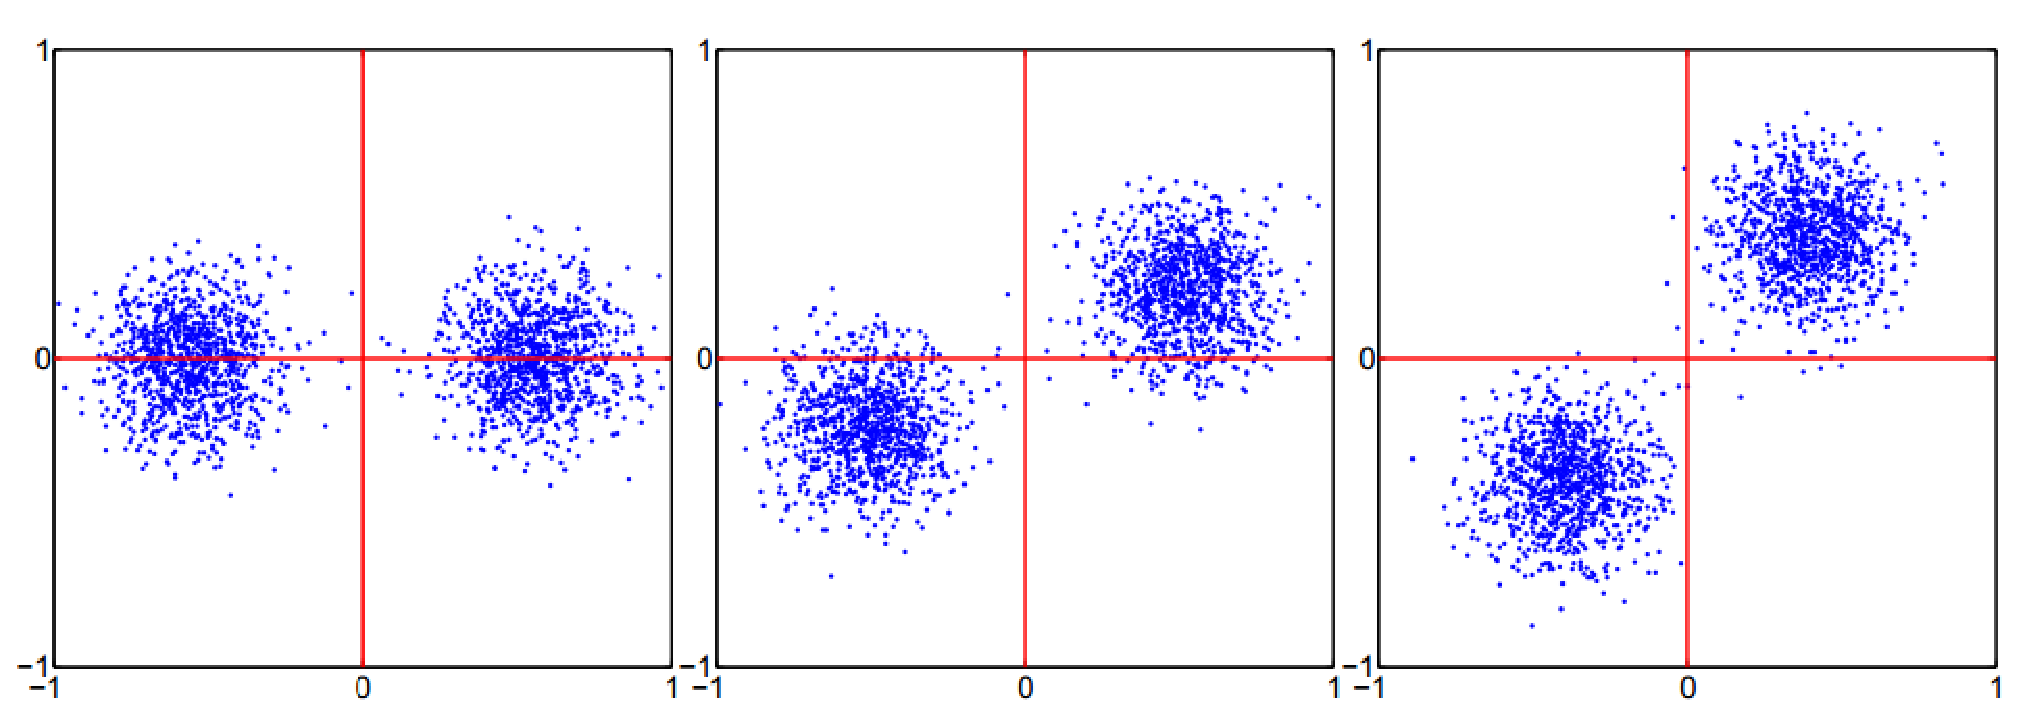
\includegraphics[width=1.0\linewidth]{itq}
  \caption{ITQ 旋转过程}
  \label{fig:itq}
  \footnotesize 注:图像来源\cite{YunchaoGong:2011:IQP:2191740.2191779}
\end{figure}
这样,整个问题的目标函数就变成了$\min \lVert B - VR \rVert_F ^2$。这个公式中有两个未知量,编码后的矩阵 $B$ 和 旋转矩阵 $R$。所以,这个问题的求解要考虑采用交替迭代的方法。先对一个随机生成的矩阵进行 SVD 分解得到一个正交矩阵作为 $R$ 的初始值,此时 $R$ 已知,就可以用$ B= \mathrm{sgn}(VR)$ 来求解 $B$;当 $B$ 已知后,可以对 $B^TV$ 进行 SVD 分解求解 $R$。既然 $R$ 求出,又可以重新一次迭代,固定 $R$ 求 $B$,如此交替迭代就可以求解出该问题。
\subsection{Cartesian K-Means}

